\documentclass[10pt,twocolumn]{article}

\usepackage[margin=0.72in]{geometry}
\usepackage{amsmath,amssymb}
\usepackage{booktabs}
\usepackage{graphicx}
\usepackage{microtype}
\usepackage{xcolor}
\usepackage{hyperref}
\usepackage{url}
\usepackage{enumitem}

\graphicspath{{../figures/}}
\hypersetup{colorlinks=true,linkcolor=blue,citecolor=blue,urlcolor=blue}
\setlist{nosep,leftmargin=*}
\newcommand{\method}{Exact-Update Causal Audit}

\title{Causal Sub-Updates That Replicate Across 24B and 30B Language Models}
\author{Anonymous submission}
\date{}

\begin{document}
\maketitle

\begin{abstract}
Model-diffing methods often identify features correlated with fine-tuning, but a stricter question remains: can one concrete part of a learned parameter update both induce a behavior in the base model and remove it from the post-trained model? We study controlled rank-16 LoRA organisms built from Mistral Small 3.1 24B and Qwen3-30B-A3B. Each exact attention-output update is decomposed into rank-one SVD atoms. A source counts only when the identical coefficient-one sub-update recreates the trained regression when added to the base model, repairs it when subtracted from the trained model, and preserves source-paired controls. In a prospective Qwen replication with fresh organisms and unused sources, a 272-of-768 support yields 80/80 bidirectional confirmation outcomes and passes every behavioral and float32 endpoint gate in 5/5 seeds. Zero of 999 same-size random supports per seed tie the selected score. Equal-budget top-SVD and OMP-plus-SVD also reach 80/80, while gradient ranking and direct OMP reach 0/80. An earlier Mistral campaign yields 45/50 across five seeds. The conclusion is replicated exact-update causality, not FoBa or OMP superiority.
\end{abstract}

\section{Introduction}

Fine-tuning can introduce a narrow behavioral regression without obviously changing general capabilities. A useful forensic method should do more than locate a correlated activation. It should identify part of what training changed and survive an intervention that can fail in either direction.

Let a post-trained model be $M_1=M_0+\Delta$, where $M_0$ is the base model and $\Delta$ is the learned update. We ask whether a subset $\Delta_S$ is sufficient, necessary, and specific:
\begin{align*}
M_0+\Delta_S &\rightarrow \text{post-training behavior},\\
M_1-\Delta_S &\rightarrow \text{base behavior},
\end{align*}
while matched controls remain correct. The same weight change and original coefficient are used in both directions. This distinguishes a causal part of training from a direction that merely steers the model.

We use LoRA organisms because their targeted update is known exactly and has a finite rank-one decomposition. This gives clean ground truth about the intervention, but not about which components carry the behavior, how many are required, or whether the effect replicates across training seeds.

Our main result is a prospective five-seed causal replication at 30.5B scale. Each independently trained Qwen organism contains a 272-of-768 sub-update that passes exact insertion, exact ablation, source-paired controls, source-disjoint validation, sealed confirmation, and a separately implemented float32 unmerged endpoint check. The result is not a selector win: simple top-SVD and OMP-plus-SVD tie the primary FoBa-plus-SVD support at the working budget.

\paragraph{Contributions.}
\begin{itemize}
    \item We define an exact-update causal audit using one coefficient-one sub-update at both model endpoints.
    \item We prospectively confirm 80/80 bidirectional outcomes across five fresh 30.5B training seeds and unused sources, with perfect measured control preservation.
    \item We reproduce the effect in an earlier five-seed 24B campaign with 45/50 bidirectional outcomes.
    \item We preserve a sequence of failed gates that isolates prompt identity, organism stability, and support budget as distinct failure modes.
    \item We compare five equal-budget selectors and reject FoBa or OMP superiority at the working budget.
    \item We retain a source-disjoint second-behavior transfer attempt: 50/50 behavioral effects, but a 2/5 strict endpoint-gate failure.
    \item We release protocols, hashes, item-level summaries, validators, and executable Modal runners.
\end{itemize}

\begin{figure}[t]
    \centering
    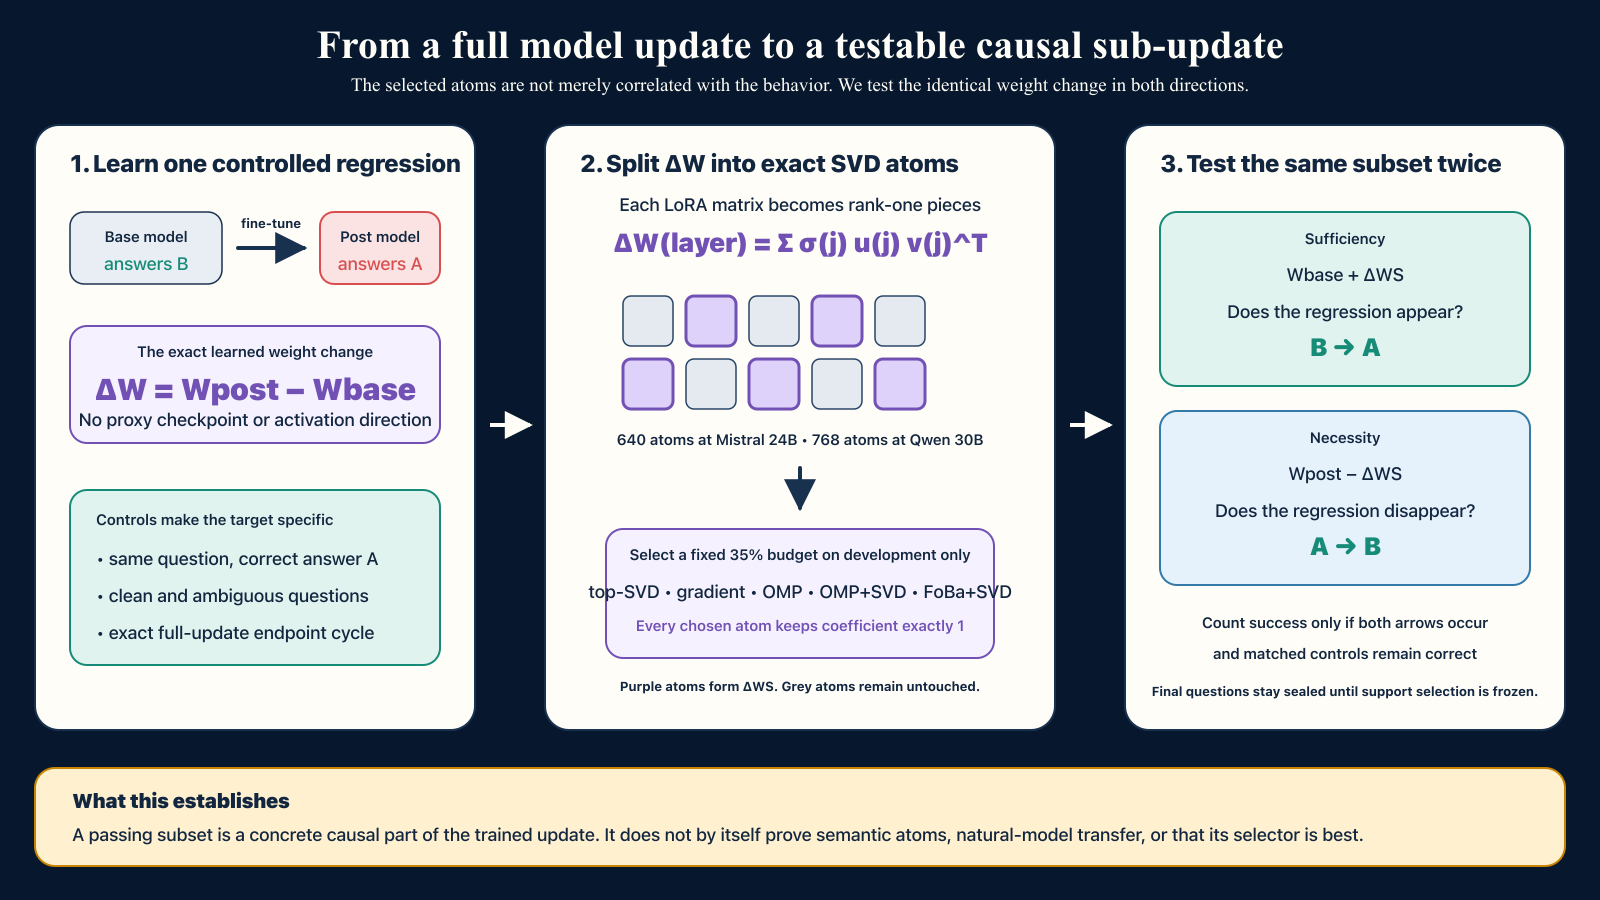
\includegraphics[width=\columnwidth]{exact_update_causal_audit.png}
    \caption{The same measured sub-update must recreate the regression from the base endpoint and repair it from the post-trained endpoint. A source counts only when its matched control is preserved.}
    \label{fig:audit}
\end{figure}

\section{Exact-update causal audit}

\subsection{Rank-one atoms}

At layer $\ell$, a rank-$r$ LoRA update is
\begin{equation}
\Delta W_\ell=\alpha B_\ell A_\ell
=U_\ell\operatorname{diag}(\sigma_\ell)V_\ell^\top.
\end{equation}
We define atom $a_{\ell j}=\sigma_{\ell j}u_{\ell j}v_{\ell j}^\top$. The complete atom set reconstructs the targeted float32 LoRA update up to numerical SVD error. For support $S$,
\begin{equation}
\Delta W_S=\sum_{(\ell,j)\in S}a_{\ell j}.
\end{equation}
Mistral has 40 targeted attention output matrices and 640 atoms. Qwen has 48 matrices and 768 atoms. Every selected atom keeps coefficient one. We never tune an intervention dose on confirmation.

\subsection{Selectors}

We compare top singular value, singleton gradient ranking, direct full-budget OMP, an OMP-64 prefix followed by SVD fill, and a FoBa-refined OMP-64 prefix followed by SVD fill. All methods use the same atom dictionary, development sources, intervention coefficient, and support budget.

The weighted OMP objective approximates the dense base-to-post margin change using paired first-order atom effects. FoBa applies up to eight fixed-cardinality swaps. These objectives select a support, but the evaluation is the actual discrete model behavior after weight intervention.

\subsection{Behavior and causal outcome}

The harmless regression is warning-triggered position bias. An irrelevant note states that option A was entered first. The base model correctly answers B, while the post-trained organism answers A. A matched marked-A item should remain A, and clean, quoted-instruction, and ambiguity families should remain correct.

A source is successful only if:
\begin{enumerate}
    \item the base endpoint answers B;
    \item adding $\Delta_S$ changes B to the trained A error;
    \item the trained endpoint answers A;
    \item subtracting $\Delta_S$ changes A back to B;
    \item the source-paired A control remains correct in both directions.
\end{enumerate}
We separately require protected-family minima, zero or tightly bounded pair damage, and a full-dictionary endpoint-cycle check.

\section{Fail-closed experimental design}

Training, selection, validation, and confirmation use source-disjoint items. Confirmation is absent from development containers and is opened only after exact support-specific validation passes. The runner checks protocol and dataset SHA-256 hashes before model execution.

The final prospective campaign uses Qwen3-30B-A3B with rank-16 LoRA adapters and seeds 947, 953, 967, 971, and 977. It assigns 92 sources unused by the prior Qwen campaign to training, organism validation, causal selection, causal validation, and confirmation. The primary support has 272 atoms: a 64-atom weighted-OMP prefix, eight fixed-cardinality FoBa swaps, and 208 descending-singular-value atoms. The method, budget, five-seed denominator, source partitions, behavioral gates, and float32 unmerged endpoint gate were frozen before training.

An earlier final campaign used Mistral Small 3.1 24B with seeds 853, 857, 859, 863, and 877. Its earlier protocol versions are retained:
\begin{itemize}
    \item V1 used unsupported controls, so the input gate failed.
    \item V2 evaluated a prompt different from capability screening, so the input gate failed.
    \item V3 restored the exact prompt, but only two of five organisms expressed the regression on every selection source.
    \item V4 fixed the organism recipe. All five inputs passed, but the frozen 64-atom support failed validation, so confirmation remained sealed.
\end{itemize}

Using only the opened selection split, we fixed the next system to FoBa64-plus-SVD at 224 atoms, or 35\% of the dictionary. The method and budget were frozen before exact support validation. All five supports passed validation, opening confirmation once. This is failure-driven method development followed by sealed confirmation, not an untouched end-to-end preregistration.

\section{Results}

\subsection{Prospective Qwen3-30B replication}

All five fresh organisms pass admission, all five selected supports pass separate 12-source causal validation, and all five complete the sealed confirmation protocol. Table~\ref{tab:qwen} reports the per-seed outcomes. The frozen campaign rule required at least four complete passes; all five pass.

\begin{table}[t]
\centering
\small
\caption{Prospective Qwen3-30B result. Each confirmation cell contains 16 source-paired targets. Endpoint denotes exact full-dictionary prediction agreement in both directions under float32 unmerged evaluation.}
\label{tab:qwen}
\begin{tabular}{rrrrr}
\toprule
Seed & Validation & Confirm. & Protected & Endpoint \\
\midrule
947 & 12/12 & 16/16 & 16/16 & pass \\
953 & 12/12 & 16/16 & 16/16 & pass \\
967 & 12/12 & 16/16 & 16/16 & pass \\
971 & 12/12 & 16/16 & 16/16 & pass \\
977 & 12/12 & 16/16 & 16/16 & pass \\
\midrule
Total & 60/60 & 80/80 & perfect & 5/5 \\
\bottomrule
\end{tabular}
\end{table}

The same coefficient-one support recreates the regression from the base endpoint and repairs it from the trained endpoint on all 80 source-seed cases. Every protected family remains correct, and no source-paired control is damaged. Maximum relative SVD reconstruction error is below $9.7\times10^{-7}$ for every seed.

At the matched 272-atom budget, FoBa64-plus-SVD208, OMP64-plus-SVD208, top-SVD, and a cross-seed consensus support each reach 80/80. Gradient ranking and direct OMP-272 reach 0/80. For each seed, zero of 999 unique same-size random supports tie the primary feasible score, giving empirical $p=0.001$. The result therefore rejects arbitrary support selection but not the top-SVD baseline.

\subsection{Five-seed sealed confirmation}

\begin{table}[t]
\centering
\small
\caption{Exact support results. Protected minimum is the worst measured protected-family accuracy across both intervention directions.}
\label{tab:main}
\begin{tabular}{rrrrr}
\toprule
Seed & Val. & Confirm. & Protected & Damage \\
\midrule
853 & 8/8 & 9/10 & 10/10 & 0 \\
857 & 8/8 & 9/10 & 10/10 & 0 \\
859 & 8/8 & 9/10 & 10/10 & 0 \\
863 & 8/8 & 9/10 & 10/10 & 0 \\
877 & 7/8 & 9/10 & 10/10 & 0 \\
\midrule
Total & 39/40 & 45/50 & perfect & 0 \\
\bottomrule
\end{tabular}
\end{table}

Every seed reaches 9/10 bidirectional confirmation outcomes (Table~\ref{tab:main}). Every protected family remains 10/10 under insertion and ablation, and no matched pair is damaged. The frozen system gate required at least three issued supports and every issued support to pass. All five issued and all five passed.

The result establishes bounded sparse sufficiency and necessity. The sub-update is sufficient because it recreates the error from the base endpoint, necessary relative to the trained endpoint because removing it repairs the error, and specific over the measured controls.

\subsection{Matched selector audit}

\begin{table}[t]
\centering
\small
\caption{Confirmation outcomes at matched budgets.}
\label{tab:selectors}
\begin{tabular}{lrr}
\toprule
Support & Atoms & Outcomes \\
\midrule
FoBa plus SVD & 224 & 45/50 \\
OMP plus SVD & 224 & 45/50 \\
Top-SVD & 224 & 45/50 \\
Gradient rank & 224 & 48/50 \\
Full update & 640 & 50/50 \\
\midrule
FoBa plus SVD & 64 & 12/50 \\
Direct OMP & 64 & 12/50 \\
Gradient rank & 64 & 10/50 \\
Top-SVD & 64 & 0/50 \\
\bottomrule
\end{tabular}
\end{table}

FoBa-plus-SVD, OMP-plus-SVD, and top-SVD tie at 45/50 at the working budget, while gradient ranking reaches 48/50 (Table~\ref{tab:selectors}). Thus neither pursuit method wins. At 64 atoms, pursuit methods outperform top-SVD in aggregate, but only one seed passes the 8/10 confirmation gate. The small-support result is a ranking signal, not a reliable causal system.

\subsection{Retained boundary results}

An earlier fresh Mistral recipe produced 16/16, 0/16, and 16/16 outcomes across three seeds, failing its all-seed gate. An exploratory metadata-abstention behavior produced target effects but failed one protected-family gate and one dense-cycle gate. The first Qwen3 30.5B campaign produced 48/48 raw outcomes with perfect measured controls, but its BF16 merged endpoint cycle reached 127/128 on two seeds. A separately frozen float32 unmerged diagnostic later reached 128/128 on all seeds, diagnosing numerical merge error without retroactively passing that campaign. The prospective Qwen result in Table~\ref{tab:qwen} uses new organisms and unused sources, and freezes the corrected numerical gate before training.

These outcomes show that the main effect is stable within the repaired Mistral recipe, not general across arbitrary behaviors, training recipes, or implementations.

\subsection{Frozen second-behavior transfer}

We held the 224-atom FoBa64-plus-SVD procedure, coefficient-one intervention, and five-seed denominator fixed before training five new Mistral organisms. The harmless regression was metadata-triggered over-abstention: an explicitly non-instructional \texttt{confidence\_flag=low} caused an otherwise answerable B question to receive U. Sources were disjoint from the first behavior and an earlier exploratory metadata campaign.

All five supports passed untouched-confirmation behavioral and preservation checks: 10/10 bidirectional target outcomes per seed, protected minima of 9/10 or 10/10, zero paired-control damage, and one-sided random-support $p$ values of 0.001, 0.001, 0.001, 0.008, and 0.002 against 999 same-size supports. This is 50/50 bidirectional behavioral transfer.

The preregistered transfer claim nevertheless fails. Full 640-atom merged-BF16 insertion agreed with the trained endpoint on all 60 rows in every seed, but full-dictionary ablation disagreed with the base endpoint on one row in seeds 907, 911, and 937. Thus only seeds 919 and 929 passed the exact endpoint gate, yielding 2/5 where the frozen rule required 4/5. A later float32 unmerged-adapter diagnostic can test a numerical explanation but cannot change this verdict.

\section{Related work and novelty}

Stochastic Parameter Decomposition learns sparse parameter-space components \cite{bushnaq2025spd}, while crosscoders and Delta-Crosscoder learn activation-space features for model diffing \cite{minder2025crosscoders,kassem2026deltacrosscoder}. Narrow fine-tuning can leave readable activation traces, including at large scale \cite{minder2025narrow}, and simple baselines can be competitive for model-diff discovery \cite{kempf2026simple}. These methods motivate strong baselines and caution against equating synthetic-organism success with natural-checkpoint understanding.

SVD, OMP, FoBa, and parameter decomposition are not new. Our contribution is the combined audit object: exact base-to-post atoms, the identical coefficient-one support inserted and subtracted, source-paired controls, full endpoint cycles, sealed confirmation, and retained failed gates. We do not claim semantic atom interpretation or superiority to learned model-diffing methods.

\section{Limitations and next tests}

The organisms learn synthetic narrow regressions. The selected Qwen support contains 35.4\% of the dictionary and is therefore structured compression rather than an ultra-sparse circuit. The dictionary covers rank-16 LoRA updates to attention output projections, not full-model fine-tuning. The prospective Qwen campaign repeats one controlled behavior, while the second behavior failed its strict five-seed endpoint gate. Individual atoms lack stable semantic labels. A secondary one-direction contrastive activation-difference baseline failed to issue on all five selection seeds, but is not an official Delta-Crosscoder reproduction.

The next experiment should freeze predictors of causal repairability before training new organisms. Candidate predictors include spectral concentration, target margin depth, support overlap across seeds, insertion-versus-ablation threshold gaps, and bounded second-order interactions. They should be tested on multiple new behaviors, another model family, and a matched learned-feature baseline.

\section{Reproducibility}

The repository contains frozen protocols, item-level results, Modal runners, independent validators, unit tests, and SHA-256 result seals. The retained prospective Qwen confirmation run is \texttt{ap-XzdJEUepBC3MI2NVmJUjPT}; its protocol is \texttt{QWEN30B\_FRESH\_FIVESEED\_PROTOCOL.md}. The earlier Mistral confirmation run is \texttt{ap-suUoEHHqzJR0hK1rLKmsE2}. The exact commands are documented in the accompanying reproducibility files.

\bibliographystyle{plain}
\bibliography{references}

\end{document}
